%# -*- coding: utf-8-unix -*-
%%==================================================
%% chapter0.tex for SJTU Master Thesis
%%==================================================


\chapter{温室CFD仿真建模与验证}
\label{chapter:CFD}
在夏季正午,由于室外气温明显高于作物的适宜生长温度,且太阳辐射量非常的大,遮阳网和自然通风已经无法完全满足温室的降温需求,此时需要通过打开风机和湿帘进行机械通风降温。虽然机械通风能实现高温条件下的有效降温,但是机械通风设备成本较高,工作能耗较大,这就要求在温室设计阶段优化温室的结构参数和设备配置,在温室运行阶段实施有效降低能耗的优化控制策略。

温室面积往往较大,为了实现有效的环境监测,通常需要较多的监测点,这将带来较高的系统监测成本,同时农业物联网的特殊性也要求监测点的数量要控制在尽量少的范围内。

温室环境是一个流场、温度场、浓度场等多个物理场耦合在一起的多输入多输出的复杂大时延系统,各个环境变量之间相互影响,且一段时间后影响效果才会得以体现,导致对温室的监测和控制分析都非常困难,本章建立了温室CFD仿真模型,并通过实验对其进行了验证,仿真结果的分析为温室监测点的选择和控制策略的制定提供了理论依据。

\section{温室CFD仿真概述}
随着计算机性能和数值计算理论水平的飞速发展,CFD越来越多地应用到各种现代科研和工程应用中,它弥补了理论分析在研究比较复杂的问题中的限制性,解决了试验研究在研究过程中的局限性,同时可以避免大型试验所带来的巨大消耗。

CFD仿真本质上是利用计算机进行数值模拟计算,完成人力所难以完成的复杂计算过程,同时结合数据可视化技术将计算结果以图形或者动画的方式展示给研究人员。CFD计算的基本思想和流程即建立流动基本方程组,然后对其进行求解,从而实现对流体流动过程的数值模拟计算。

温室内是一个非常复杂的环境,多个物理场相互耦合在一起共同作用,不仅受到温室内外环境的变化的影响,还与温室的结构和作动器的动作有着密切的关系,且温室是一个大时延的系统,温室往往需要经过一段时间后,才会对环境变化或作动器动作有所反应。因此仅仅依靠传统的理论方法和试验方法难以解决温室内复杂的流场问题,CFD技术的发展,为温室内流场问题的研究带来了新的方法和手段。

OKUSHIMA等首次应用CFD研究温室的通风问题,开拓了定量分析温室通风问题的有效途径。此后,随着CFD理论的不断完善和商用CFD软件的发展,温室通风CFD仿真结果已被证明具有良好的吻合性,计算速度也越来越满足生产的需要,研究效率大大提高。目前,CFD仿真已经成为进行温室通风研究的常用方法。

在基于CFD的机械通风研究领域,随着仿真技术的发展和问题分析的深入,模型由二维到三维全尺度,由稳态分析到瞬态分析,由简单模拟到用于优化控制设计。BOURNETA等采用CFD方法研究了风机形状和安装方式对于温室内流体流动分布情况的影响。童莉等建立了机械通风条件下的温室三维CFD模型,研究了温室气温可控距离与入口风速和湿帘安装高度之间的关系。CHEN等采用CFD方法研究了湿帘、风机安装位置与湿帘-风机系统降温效果之间的关系。胥芳等采用CFD 方法分析了不同温室长度、湿帘入口面积和风机转速对于温室降温的影响,并根据分析结果提出了优化方案。任守纲等基于CFD方法建立了夏季温室气温变化瞬态模型,研究了自然通风和机械通风降温措施切换控制策略。

通过本文设计实现的智能温室监测与控制系统,使得根据当前温室内外的环境参数对温室机械通风实时控制成为可能,从而更有效地提高机械通风效率、降低运行能耗。在温室机械通风实施优化控制的过程中,需要选择合理的监测点位置,获取机械通风效果与各工作参数之间的定量关系。由于实际工作环境的不可重复性,温室CFD仿真比实验能更有效地确定机械通风效果与控制参数之间的关系。温室机械通风是典型动态过程,但目前对于机械通风瞬态过程的实验和仿真研究还不够深入,因此本文建立全尺度三维瞬态和稳态CFD仿真模型,反映机械通风作用下,温室内空气温度的时空分布和变化过程,用以评价机械通风效果、选择合适的监测点位置方案、优化风机的控制策略。


\section{温室环境CFD建模}
	\subsection{理论基础}
		\subsubsection{基本控制方程}
所有的流体流动都遵循基本的守恒定律,包括质量守恒定律、动量守恒定律、能量守恒定律,对于多组分的流体流动还需要遵循组分守恒定律。

自然任何自然现象,包括流体流动,都满足质量守恒定律,由质量守恒定律可以得到质量守恒方程,也称为连续性方程,如式\ref{eqn:zhiliang}所示:
	\begin{equation}
		\label{eqn:zhiliang}
		\frac{\partial\rho}{\partial t}+\frac{\partial \rho u}{\partial x}+\frac{\partial \rho v}{\partial y}+\frac{\partial \rho w}{\partial z}=0
	\end{equation}

引入散度符号$\nabla$可表示为式\ref{eqn:zhiliang1}
	\begin{equation}
		\label{eqn:zhiliang1}
		\frac{\partial\rho}{\partial t}+\nabla \cdot (\rho \mathbf{u}) =0
	\end{equation}
其中$\rho$为流体密度,$t$为时间,$\mathbf{u}$为速度矢量。

对于不可压流体,密度$\rho$可看作常数,可得式\ref{eqn:zhiliangRho};对于稳态流动,密度$\rho$不随时间变化,可得式\ref{eqn:zhiliangRhoCon}。
	\begin{equation}
		\label{eqn:zhiliangRho}
		\nabla \cdot \mathbf{u} =0
	\end{equation}
	\begin{equation}
		\label{eqn:zhiliangRhoCon}
		\nabla \cdot (\rho \mathbf{u}) =0
	\end{equation}
动量守恒定律也是任何流体流动都必须遵循的基本物理定律,由该定律可得$x$、$y$、$z$三个方向的动量守恒方程如式(5)所示:
	\begin{equation}
		\label{eqn:dongliang}
		\left\{
		\begin{aligned}
		\frac{\partial \rho u}{\partial t}+\nabla \cdot (\rho u \mathbf{u}) = - \frac{\partial \rho}{\partial x}+\frac{\partial \tau_{xx}}{\partial x}+\frac{\partial \tau_{yx}}{\partial y}+\frac{\partial \tau_{zx}}{\partial z} + F_x \\
		\frac{\partial \rho v}{\partial t}+\nabla \cdot (\rho v \mathbf{u}) = - \frac{\partial \rho}{\partial y}+\frac{\partial \tau_{xy}}{\partial x}+\frac{\partial \tau_{yy}}{\partial y}+\frac{\partial \tau_{zy}}{\partial z} + F_y \\
		\frac{\partial \rho w}{\partial t}+\nabla \cdot (\rho w \mathbf{u}) = - \frac{\partial \rho}{\partial z}+\frac{\partial \tau_{xz}}{\partial x}+\frac{\partial \tau_{yz}}{\partial y}+\frac{\partial \tau_{zz}}{\partial z} + F_z 
		\end{aligned}
		\right.
	\end{equation}
其中$p$为流体微元体上的压力,$\tau_{ii}$为作用在微元体表面上的黏性应力的分量,$F_x$、$F_y$、$F_z$为微元体上的体积力,在只存在重力的情况下,且规定$z$轴竖直向上时,则有$F_x=0$、$F_y=0$、$F_z=\rho g$。

对于牛顿流体,黏性应力与流体的变形率成比例,可得如下动量守恒方程,即著名的Navier-Stokes(N-S)方程,如式(6)所示:
	\begin{equation}
		\label{eqn:ns}
		\left\{
		\begin{aligned}
		\frac{\partial \rho u}{\partial t}+\nabla \cdot (\rho u \mathbf{u}) =- \frac{\partial \rho}{\partial x}+\nabla \cdot (\mu \nabla \cdot u ) + S_x \\
		\frac{\partial \rho v}{\partial t}+\nabla \cdot (\rho v \mathbf{u}) =- \frac{\partial \rho}{\partial y}+\nabla \cdot (\mu \nabla \cdot v ) + S_y \\
		\frac{\partial \rho w}{\partial t}+\nabla \cdot (\rho w \mathbf{u}) =- \frac{\partial \rho}{\partial z}+\nabla \cdot (\mu \nabla \cdot w ) + S_z 
		\end{aligned}
		\right.
	\end{equation}
其中,$\mu$为动力黏度,$S_x$、$S_y$、$S_z$为方程的广义源项,有 $S_x=F_x+s_x$、$S_y=F_y+s_y$、$S_z=F_z+s_z$,一般情况下,$s_x$、$s_y$、$s_z$都为小量,对于不可压流体,$s_x=s_y=s_z=0$。

对于存在能量交换的物理问题还必须遵循能量守恒定律,存在能量交换的流体流动问题也是如此,由该定律可得能量守恒方程,对于牛顿流体,如式(7)所示:
	\begin{equation}
		\label{eqn:heat}
		\rho C_p (\frac{\partial T}{\partial t}+(\mathbf{u} \cdot \nabla) T + \nabla \cdot \mathbf{q}  =Q
	\end{equation}
其中$C_p$为恒压比热容,$T$为热力学温度,$\mathbf{q}$为热通量矢量,$Q$为能量源项。

对于存在物质交换的流体流动问题中,每种组分还必须要满足组分守恒定律,由该定律可得组分守恒方程,如式(8)所示:
	\begin{equation}
		\label{eqn:conc}
		\frac{\partial c_i}{\partial t}+\mathbf{u} \cdot \nabla c_i = \nabla \cdot (D_i \nabla c_i ) + R_i
	\end{equation}
其中$c_i$为组分$i$的浓度,$D_i$为组分$i$的扩散系数,$R_i$为单位时间内系统内单位体积通过化学反应生成的组分$i$的量。
		\subsubsection{温室流体流动问题的简化}
研究表明,对于气体流速较小,一般为50 m/s以下,压强梯度不大时,气体流体可以看作不可压流体。通常情况下,温室内植物生产区域的气流速度不宜过高,一般低于2 m/s,因此温室中的流体为低速流动,可看作不可压流体。另外,在仿真中可以假设温室内气体为连续、稳定的牛顿流体,并忽略黏性发热和压力功。而且一般可假设气体的各组分之间无化学反应。

		\subsubsection{湍流模型的选择}
湍流是一种即使边界条件不发生变化,流动也处于不稳定的状态,各个流动相关的变量随机发生变化。根据流动实验结果,当雷诺数(Reynolds数,简称Re数)大于另一个临界值时,流体流动将变得混乱,出现不同尺度的涡,此时流体流动为湍流。

在温室内,由于温室尺寸往往较大,温室内流体流动的Re数较大,根据相关文献,温室内自然对流即呈现出湍流状态,机械通风情况下Re数更大,更加呈现出高度湍流。因此,在温度分布不均匀和机械通风的共同作用下,以及流体受边界的限制,温室内的气体流动可看作是湍流流动。

对于湍流的数值计算目前有直接数值计算和非直接数值计算两种。

直接数值计算即为直接用流动控制方程对湍流进行求解计算,可以得到最真实的理论解,得到的结果也是最精确的,但是该方法对于计算机的性能要求非常高,目前只能用来求解比较简单的问题,对于复杂的工程问题还不具有现实工程意义。

目前,非直接数值计算对于解决实际工程问题使用最为广泛的为Reynolds平均法,该方法可以用相对小的计算量得到相对精确的计算结果。

本文选用工程上广泛使用的Reynolds平均法中的标准 湍流模型进行温室通风仿真。该模型引入了湍动能 方程,如式(9)所示,和湍流耗散率 方程,如式(10)所示。
	\begin{equation}
		\label{eqn:k}
		\rho \frac{\partial k}{\partial t}+\rho \mathbf{u} \cdot \nabla k = \nabla \cdot ((\mu + \frac{\mu_t}{\sigma_k}) \nabla k) -\rho \varepsilon +P_k
	\end{equation}
	\begin{equation}
		\label{eqn:e}
		\rho \frac{\partial \varepsilon}{\partial t}+\rho \mathbf{u} \cdot \nabla \varepsilon = \nabla \cdot ((\mu + \frac{\mu_t}{\sigma_{\varepsilon}}) \nabla \varepsilon ) +C_{\varepsilon 1} \frac{\varepsilon}{k} P_k - C_{\varepsilon 2} \rho \frac{\varepsilon^2}{k}
	\end{equation}
其中$C_{\mu}$、$C_{\varepsilon 1}$、$C_{\varepsilon 2}$、$\sigma_k$、$\sigma_{\varepsilon}$为常数,$\mu_t =\rho C_{\mu} \frac{k^2}{\varepsilon}$,
$P_k=\mu_t(\nabla \mathbf(u):(\mathbf(u)+(\mathbf(u))^T))-\frac{2}{3}(\nabla \mathbf(u))^2)-\frac{2}{3}\rho k \nabla \cdot \mathbf(u)$。

但是标准 湍流模型是针对充分发展的湍流流动建立的,不适用于湍流发展不充分的近壁面区域,因此需要引入壁面函数法解决该问题。壁面函数法即在湍流核心区采用标准 湍流模型求解,而在壁面区借助一组半经验公式,将壁面区与核心区的求解变量关联起来,这样不用对壁面区进行求解也可以得到与壁面区域相邻节点的变量值了。
	\subsection{仿真软件}
	目前对于CFD仿真计算,比较常见的计算仿真软件有FLUENT、CFX、COMSOL Multiphysics等,但是FLUENT、CFX等均作为CFD计算求解器存在,还需要配合GAMBIT等前处理软件和TECPLOT等后处理软件使用,COMSOL Multiphysics提供整个流程的解决方案,几何建模、前处理、求解和后处理之间无缝结合,因此本文CFD仿真使用COMSOL Multiphysics 5.2作为仿真软件。
	
COMSOL Multiphysics是当今世界第一款真正的任意多物理场直接耦合分析软件,计算快速高效精确,采用完全开放的架构,可以轻松地自定义专业的偏微分方程,而无需使用复杂的UDF开发,可以实现任意求解参数的独立函数控制,拥有丰富的后处理功能,可以根据需要进行任意数据、曲线、图片及动画的生成及导出,且支持跨平台计算和并行计算。

	\subsection{几何建模}
本文CFD仿真研究对象为我国南方典型连栋塑料温室,位于上海市崇明岛(E121.74°,N31.50°),温室如\ref{fig:House}所示。
	\begin{figure}[!htp]
		\centering
		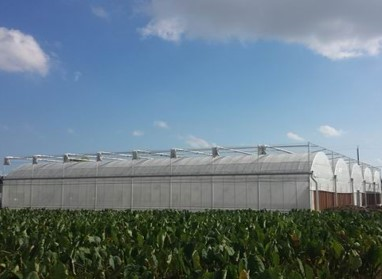
\includegraphics[width=0.3\textwidth]{15House.png}
		\bicaption[fig:House]{南方连栋塑料温室}{南方连栋塑料温室}{Fig}{Multi-span plastic greenhouse in Southern China}
	\end{figure}
温度顶高5 m,肩高3 m,屋脊方向为东西走向,长度32 m,单栋跨度8 m,共5栋,总宽度40米。温室西墙安装湿帘,湿帘高度为1.8 m,中心位置安装高度为1.3 m,每套长度为17 m,温室南北两侧各一套,中间为2 m宽的推拉门。温室东墙安装10台YS1250型重锤式负压风机,每栋两台,风机直径为1250 mm,中心位置安装高度为1.5 m,电机功率为1.1 kW,单台排风量 为40000 m3/h。温室主体采用结构钢,四周及顶部覆盖聚乙烯薄膜,薄膜厚度为0.15 mm,透光率大于(等于)90%,顶部安装遮阳网,采用专用优质缀铝外遮阳网布,遮阳率可达80\%。

在COMSOL Multiphysics中按照1:1的比例建立温室的几何模型,如\ref{fig:Geometrical}所示。
	\begin{figure}[!htp]
		\centering
		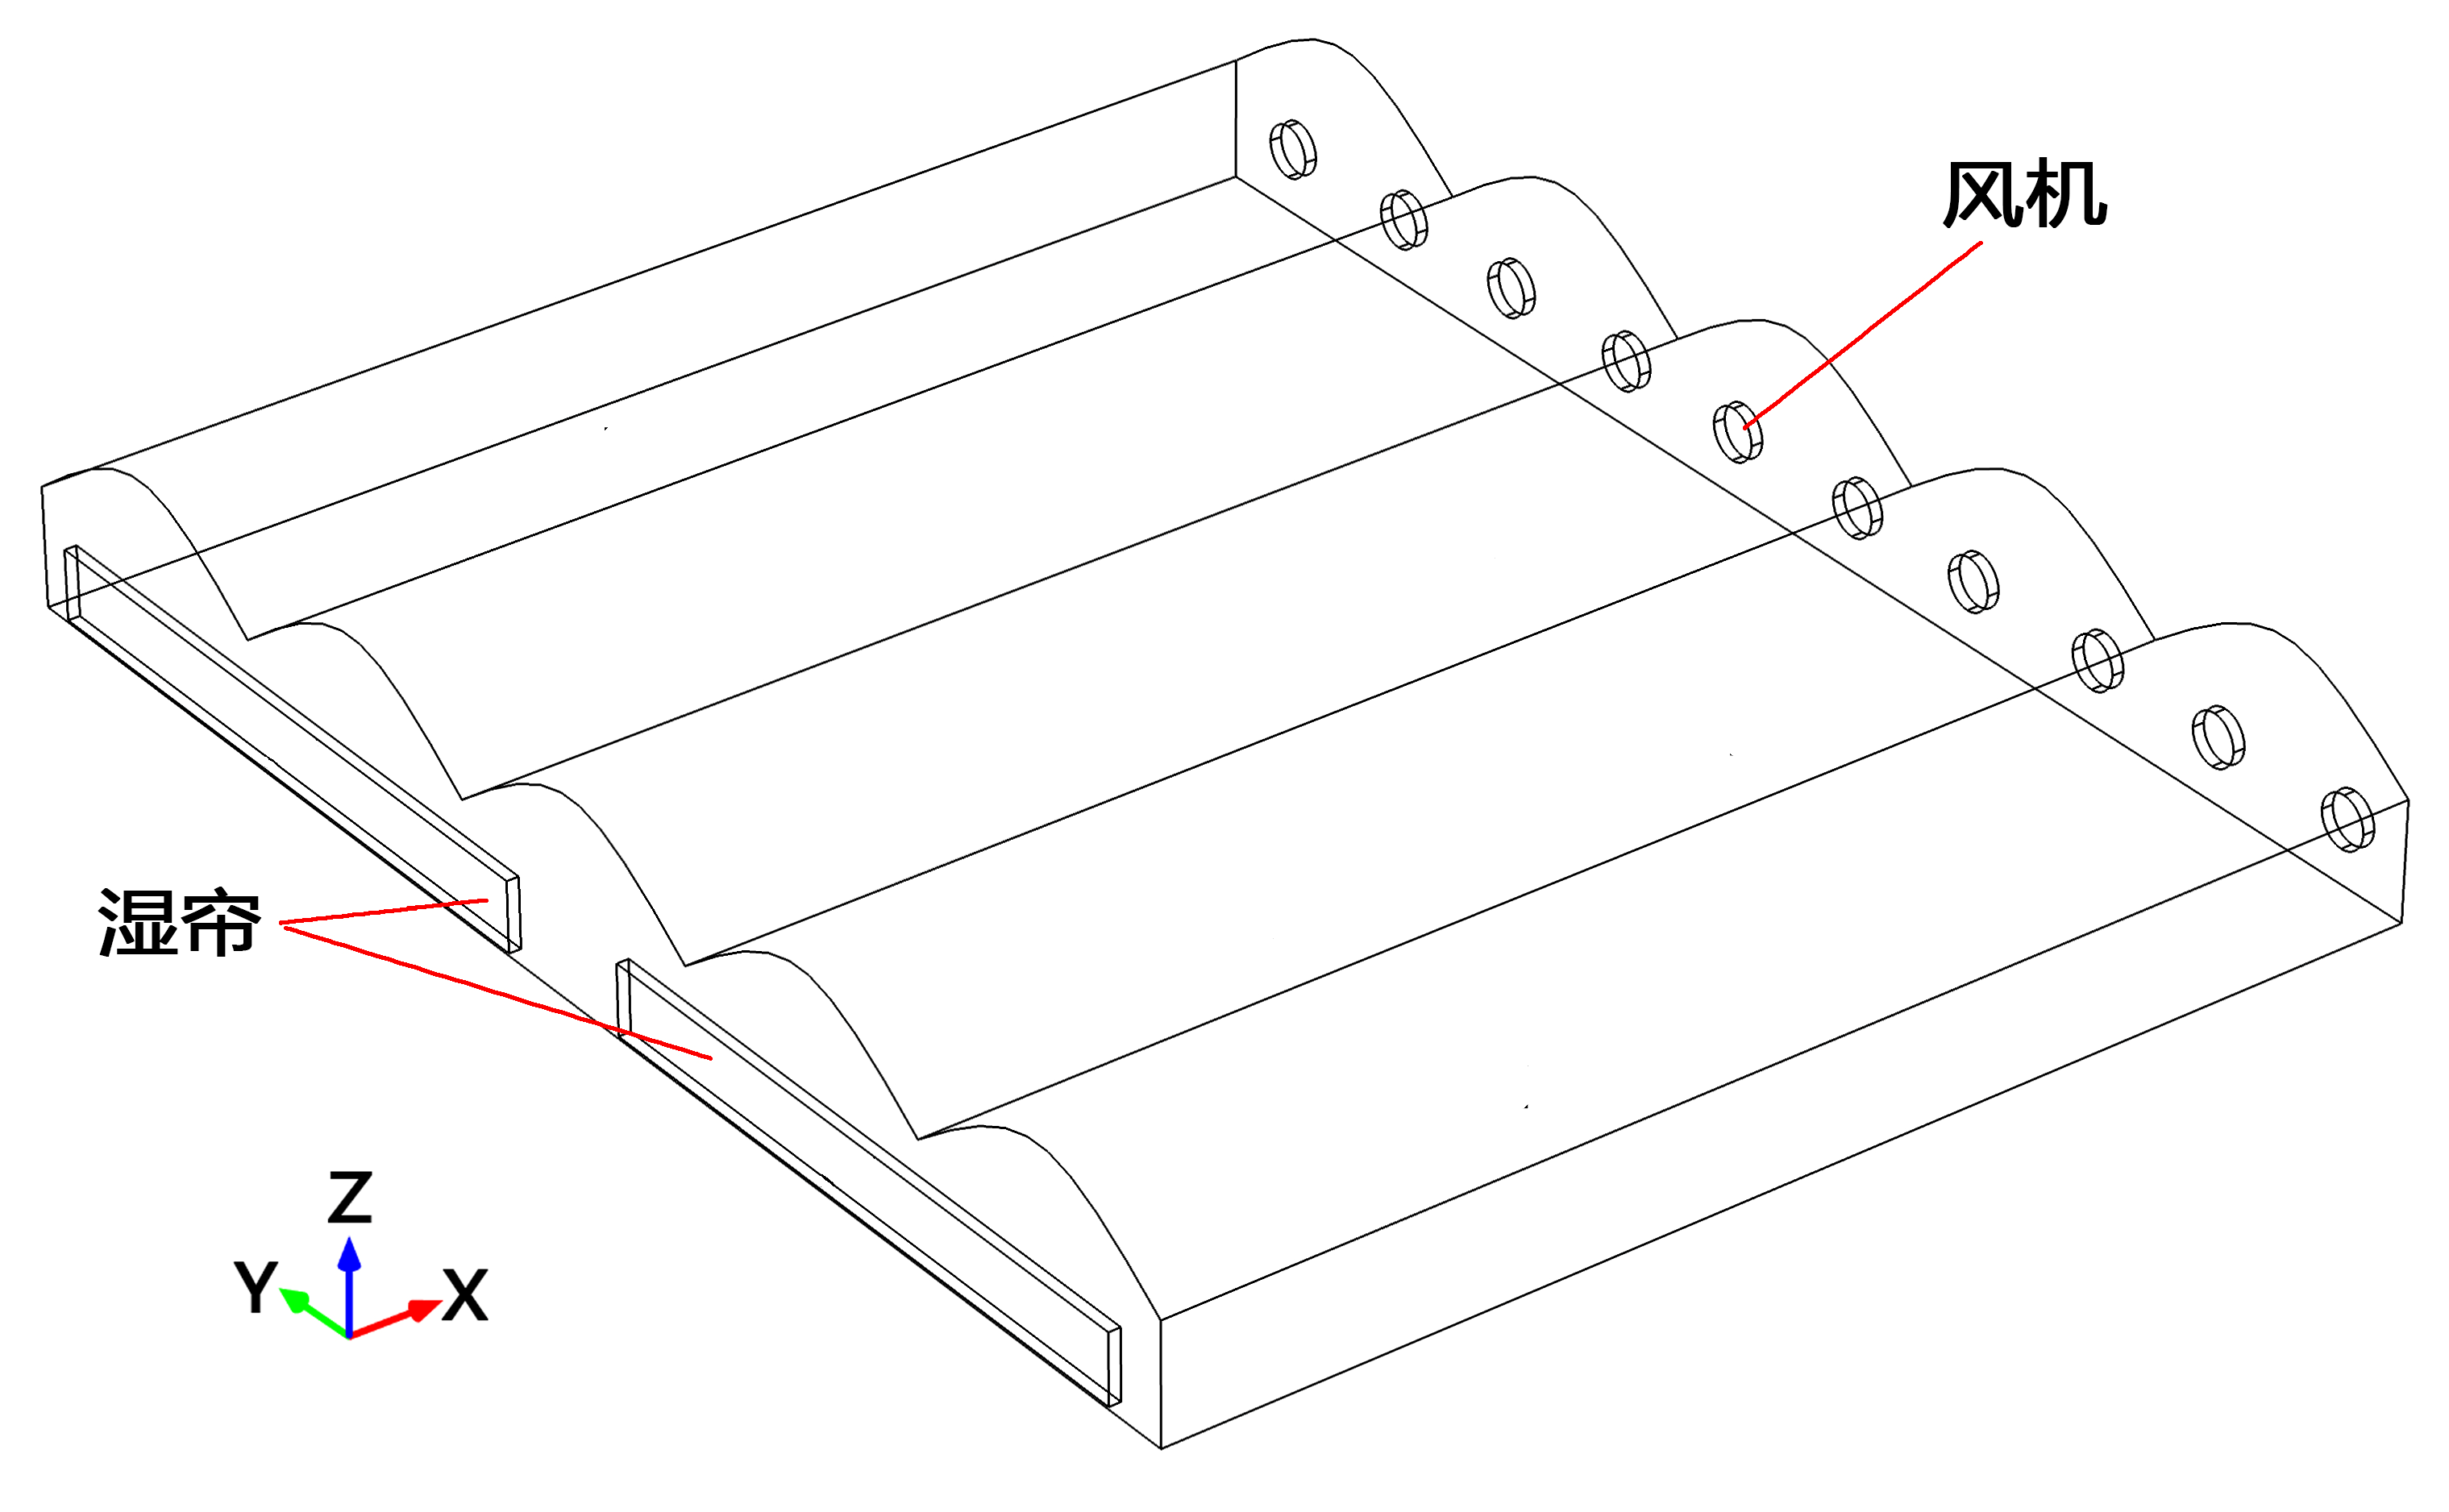
\includegraphics[width=0.7\textwidth]{16Geometrical.png}
		\bicaption[fig:Geometrical]{温室几何模型}{温室几何模型}{Fig}{Geometrical model of the greenhouse}
	\end{figure}
本模型为减少计算量,提高计算速度,根据研究侧重点和温室特点对温室几何模型做出如下合理的简化:
	\begin{enumerate}
		\item 温室表面的薄膜厚度仅有0.15 mm,在模型中可以忽略不计,因此几何模型中简化为无厚度的面。
		\item 由于侧窗、顶窗和门在机械通风过程中均为关闭状态,对温室机械通风过程不起作用,且会增加网格数量,同时影响网格的划分质量,因此几何模型忽略了它们的细节建模。
		\item 温室内的支撑结构和排水沟相较温室尺寸较小,对通风过程影响较小,且会急剧增加网格的数量,使计算速度缓慢,因此在建模过程中忽略。
		\item 温室外遮阳网通过太阳辐射强度折减来体现,不体现在几何模型中。
		\item 实验期间温室内种植高度低于20 cm的西瓜和甜瓜,因此忽略其几何建模。
	\end{enumerate}
	
	\subsection{多物理场}
	机械通风条件下,温室内气温的时空分布和变化受室内外环境条件、湿帘-风机、太阳等因素的影响。因此,需要在COMSOL中添加多个物理场模块。
	
首先为解决流场问题,在软件中流体流动模块下添加单相流-湍流-湍流, 模块;然后因为温室仿真中涉及到流体传热,在软件中传热模块下添加流体传热模块;最后考虑到湿帘和水分蒸发对于温室中环境的影响,在软件中化学物质传递模块下添加稀物质传递模块。

为建立各个物理场模块之间的耦合关系,对各个模块之间做如下处理:
	\begin{enumerate}
		\item 湍流模块和稀物质传递模块之间通过速度、绝对压力和浓度耦合;
		\item 湍流模块和流体传热模块之间通过速度、绝对压力和温度耦合;
		\item 稀物质传递模块和流体传热模块之间通过浓度耦合。
	\end{enumerate}
为了引入流体传热模块对流体密度和黏度的影响,在多物理场选项下添加非等温流模块。

	\subsection{边界条件}
	为获得温室机械通风过程的初始状态,从而研究机械通风过程及其升温过程,本文仿真过程分为湿帘风机关闭状态和开启状态。前者温室处于密闭环境,风机和湿帘处于关闭状态,用以计算自然对流状态下温室内的状态;后者风机和湿帘处于开启状态,进行机械通风过程仿真,用以计算湿帘风机对温室内环境分布和变化的影响。
	
本次仿真以温室内的空气为主要研究对象,所涉及的边界条件包括室外环境参数、温室四周薄膜和顶棚、风机、湿帘、室内地面等,设置见\ref{tab:boundary}。由于关注的仿真过程时间较短,故可以忽略在此期间内各边界条件基本参数的变化,各算例基本参数设置见\ref{tab:basicParameters}。
		\begin{table}[!hpb]
  			\centering
  			\bicaption[tab:boundary]{CFD模型边界条件}{CFD模型边界条件}{Table}{Boundary condition used in the CFD model}
  			\begin{tabular}{ccccc} \toprule
			类型	 & 边界 & 湍流场 & 	流体传热 & 	稀物质传递\\ \midrule
			\multirow{5}{*}{关闭风机} & 四周围护 & 壁面 & 热通量、散射面 & 无通量\\ 
												  & 顶棚  & 壁面 & 热通量、散射面 & 无通量\\
												  & 地面 & 壁面 & 温度、散射面 & 无通量\\
												  & 风机 & 壁面 & 热通量、散射面 & 无通量\\
												  & 湿帘 & 壁面 & 热通量、散射面 & 无通量\\ \midrule
			\multirow{5}{*}{开启风机} & 四周围护 & 壁面 & 热通量、散射面 & 无通量\\
												  & 顶棚 & 壁面	 & 热通量、散射面	 & 无通量\\
												  & 地面 &  壁面 & 温度、散射面	 & 无通量\\
												  & 风机 &  压力出口 & 	流出 & 	流出\\
												  & 湿帘 & 速度入口	 & 温度 & 浓度\\ \bottomrule
 			\end{tabular}
		\end{table}	
		\begin{table}[!hpb]
  			\centering
  			\bicaption[tab:basicParameters]{基本参数设置}{基本参数设置}{Table}{Common parameters in the CFD model}
  			\begin{tabular}{cc} \toprule
			参数 & 数值\\ \midrule
			太阳辐射强度/(W·m-2) & 	832\\
			室外环境温度/℃	 & 36.5\\
			室内地面温度/℃ & 	39.5\\
			入口相对湿度/\%	 & 82.3\\
			薄膜壁面温度/℃	 & 39.5\\
			薄膜顶棚温度/℃	 & 41.5\\
			薄膜对流换热系数/(W·(m2·K)-1) & 6.6\\
			土壤发射率 & 0.92\\
			薄膜发射率 & 0.7\\
			土壤吸收率 & 0.88\\
			薄膜吸收率 & 0.1\\ \bottomrule
 			\end{tabular}
		\end{table}
湿帘风机关闭状态下,即计算自然对流状态时,还需对温室整个计算域设置体积力域,用以计算空气密度因为受温度变化影响而带来的自然对流,并设置压力约束点以提供压力参考点。

湿帘风机开启状态下,即计算机械通风过程时,入口风速计算见式\ref{eqn:input}:
	\begin{equation}
		\label{eqn:input}
		v_{in} = \frac{n Q_{fan}}{S_{in}}
	\end{equation}
其中$v_{in}$为入口风速,$n$为开启风机的数量,$Q_{fan}$为单台风机的排风量,$S_{in}$为湿帘入口总面积。

入口温度可根据湿帘降温模型计算见式\ref{eqn:cool}:
	\begin{equation}
		\label{eqn:cool}
		T_{in}=T_{out}-E (T_{out} - T_{w})
	\end{equation}
其中$T_{in}$为湿帘后干球温度,$T_{out}$为湿帘前干球温度,$E$为湿帘蒸发冷却换热效率,$T_w$为湿帘前湿球温度。

	\subsection{网格划分和求解步骤}
为研究机械通风条件下,整个温室内的空气温度时空分布和变化,本文CFD仿真计算选取整栋温室作为计算域。模型内部大部分区域采用自由剖分四面体网格进行划分,并在入口、出口和壁面边界处进行边界层加密,以适应该区域速度、温度和浓度梯度变化大的要求。为得到数值计算的网格无关解,反复尝试不同密度的网格,本次计算整个模型共划分743604域单元、59854边界单元和 2424边单元,如\ref{fig:Mesh}所示。
	\begin{figure}[!htp]
		\centering
		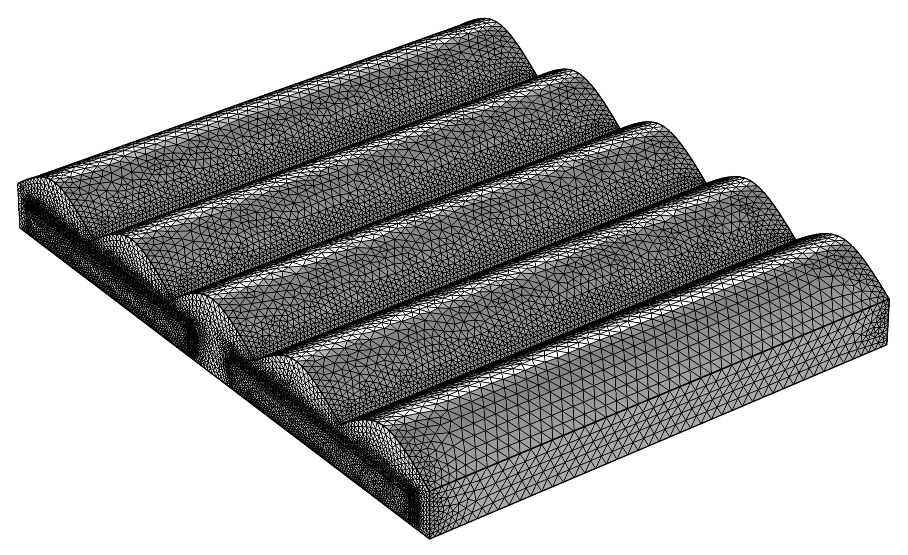
\includegraphics[width=0.5\textwidth]{17Mesh.png}
		\bicaption[fig:Mesh]{温室CFD模型网格划分}{温室CFD模型网格划分}{Fig}{Mesh of the greenhouse CFD model}
	\end{figure}
本次仿真计算划分为若干个阶段:

第1阶段进行湿帘风机关闭状态下的稳态求解,此阶段用以计算自然对流状态下温室内状态分布,为进行机械通风的仿真计算获得初始值,此阶段使用稳态求解器进行求解;

第2阶段进行湿帘风机开启状态下的瞬态求解,求解变量的初始值设为第1阶段的计算解,此阶段使用瞬态求解器进行求解;

随后每个阶段都以上阶段的计算结果作为初始值进行稳态或瞬态任意状态的仿真计算。各阶段之间的求解计算主要关注速度、绝对压力、温度、浓度等关键参数的传递。

本文所有CFD仿真计算均在Intel Xeon E5-1620V3 四核心CPU,主频3.5GHz,内存64GB,操作系统为Windows10 x64的小型工作站上进行,CFD仿真建模过程中前处理、求解、后处理等过程均在COMSOL Multiphysics 5.2环境下进行。各算例稳态计算历时近6 h完成,瞬态计算与仿真步长和时长有关,如步长1.5 s时长10 min历时近15 h完成。

\section{机械通风实验}
	\subsection{实验平台}
本次实验的实验平台为本文设计并实现的智能温室系统,通过该系统平台实现室内的空气温湿度、土壤温湿度的测量,和室外的空气温湿度、太阳辐射强度等的测量。
	
部分无需长期监测的数据如土壤表面温度和薄膜表面温度,本次实验采用单独的设备进行测量。土壤表面温度的测量采用CA380型手持红外测温仪,测量范围为-32~380℃,测量精度为±2℃;薄膜表面温度测量采用铂电阻PT100,测量范围为-200~200℃,测量精度为±0.15℃。

	\subsection{实验方案}
一般情况下,七月下旬至八月上旬,上海地区的气温达到全年的最高值,该段时间内对于温室的降温尤为重要。本次实验的实验时间为2016年7月31日,天气晴朗,室外温度较高且相对平稳。实验开始时间为13:10,温度为一天中最高的阶段,室外气温达到36℃以上,此时仅依靠自然通风等手段已经无法将温度降至32℃以下。研究表明,室内气温达到32℃以上将对作物的生长产生较大的影响,此时需要开启湿帘-风机进行机械通风降温。实验期间温室外遮阳网保持打开。
	\begin{figure}[!htp]
		\centering
		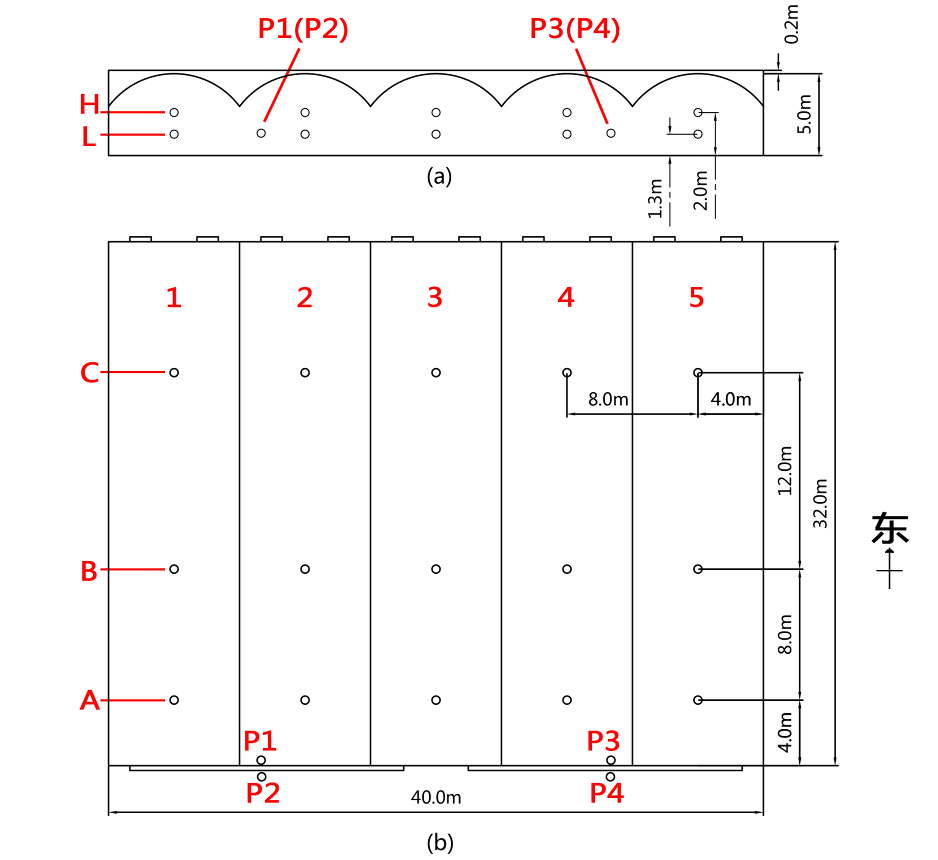
\includegraphics[width=0.7\textwidth]{18Distribution.png}
		\bicaption[fig:Distribution]{温室内传感器节点分布图}{温室内传感器节点分布图}{Fig}{Distribution of sensors in the greenhouse}
	\end{figure}
实验期间,温室内所有传感器测点每20 s记录一次数据。温室内外共布置30个测量节点,具体分布如\ref{fig:Distribution}所示。传感器编号方式如\ref{fig:Distribution}所示,距离湿帘4、12、24 m位置处分别编号A、B、C,距离地面1.3 m和2 m位置处分别编号H、L,自北向南每栋编号1、2、3、4、5,除HA1、HC1、HA5、HC5外,其余位置各布置一个节点;另外分别在紧邻湿帘内外正中间位置处,东西两侧各布置一个节点,如\ref{fig:Distribution}所示的P1、P2、P3、P4点。为避免温室等建筑物对于室外气象站的影响,室外气象站布置在距离温室10 m处的空旷区域,安装在距离地面10 m处的位置,距离温室较远且体积较小,因此未在图中标出。

	\subsection{实验步骤}
根据实验方案,本次实验分别进行了开启关闭10台、6台和4台风机的机械通风实验。
	
每组实验采用相同的实验步骤:
	\begin{enumerate}
		\item 实验前的准备工作,检查所有实验设备,确保所有设备正常工作,完成温室的密封性检查,并将温室缝隙补上。
		\item 关闭所有门窗,待温室内气温升高至稳定。
		\item 打开湿帘处的卷帘,开启风机,待温室内气温降低至稳定。
		\item 关闭风机,关闭湿帘处的卷帘,待温室内气温升高至稳定。
		\item 重复上述步骤,进行下一组实验。
	\end{enumerate}
	
	\subsection{实验结果}
	本文选取最具代表性的先后开启和关闭10台和4台风机情况下植物冠层即截面L典型位置处的实验结果进行分析,实验测得的温室内气温变化曲线如图23所示。
	\begin{figure}[!htp]
		\centering
		\subfigure[截面2温度实测值]{
			\includegraphics[width=0.8\textwidth]{result/01.png}
		}
		\subfigure[截面B温度实测值]{
			\includegraphics[width=0.8\textwidth]{result/02.png}
		}
		\subfigure[风机开启情况]{
			\includegraphics[width=0.8\textwidth]{result/03.png}
		}
 		\bicaption[fig:Result]{温室内植物冠层温度实测值}{温室内植物冠层温度实测值}{Fig}{Measured temperature inside the greenhouse at Section L}
 	\end{figure}
	如\ref{fig:Result}所示,由实验结果曲线可以看出,对于开启10台和4台风机的情况,各测点空气温度变化趋势基本一致,即开启风机时首先快速下降,随后缓慢下降,最后达到最低温度,并保持稳定。两者的差别体现在,开启10台风机的情况下,相较于开启4台风机的情况,空气温度下降速度较快,且纵向温度梯度较大,最终达到的稳定温度略低,横向分布较为均匀。关闭风机后,两种情况的空气温度上升趋势基本一致。
	
图\ref{fig:Result}所示为屋脊方向典型纵截面,即如\ref{fig:Distribution}所示截面2的实验结果,该截面的结果可以观察到与湿帘不同距离测点空气温度的变化情况,从结果中可以看出距离湿帘越近,空气温度下降越早,且最终达到的稳定温度越低。

图\ref{fig:Result}所示为温室跨度方向典型横截面,即如\ref{fig:Distribution}所示截面B的实验结果,该截面的结果可以观察到每栋内测点空气温度的变化情况,可以看出受推拉门处造成的湿帘不连续的影响,第3栋降温效果最差,空气温度下降速度最慢,且最终达到的稳定温度最高。

\section{模型验证}
模型验证时选取实验参数作为边界条件参数,具体参数见\ref{tab:cases}中Case 1的参数设置,即开启风机数量为10台,入口温度为30℃,温室长度为32 m,其它基本参数设置如表5所示。实验条件下,温室内植物冠层即截面L的典型截面即截面2和截面B中的各测点空气温度仿真值和实测值如图24所示,由于截面B具有对称性,因此图中仅展示B1、B2、B3测点结果。
	\begin{figure}[!htp]
		\centering
		\subfigure[截面2仿真值]{
			\label{fig:Compare:a}
			\includegraphics[width=0.4\textwidth]{compare/01.png}
		}
		\subfigure[截面2实测值]{
			\label{fig:Compare:b}
			\includegraphics[width=0.4\textwidth]{compare/02.png}
		}
		\subfigure[截面B仿真值]{
			\label{fig:Compare:c}
			\includegraphics[width=0.4\textwidth]{compare/03.png}
		}
		\subfigure[截面B实测值]{
			\label{fig:Compare:d}
			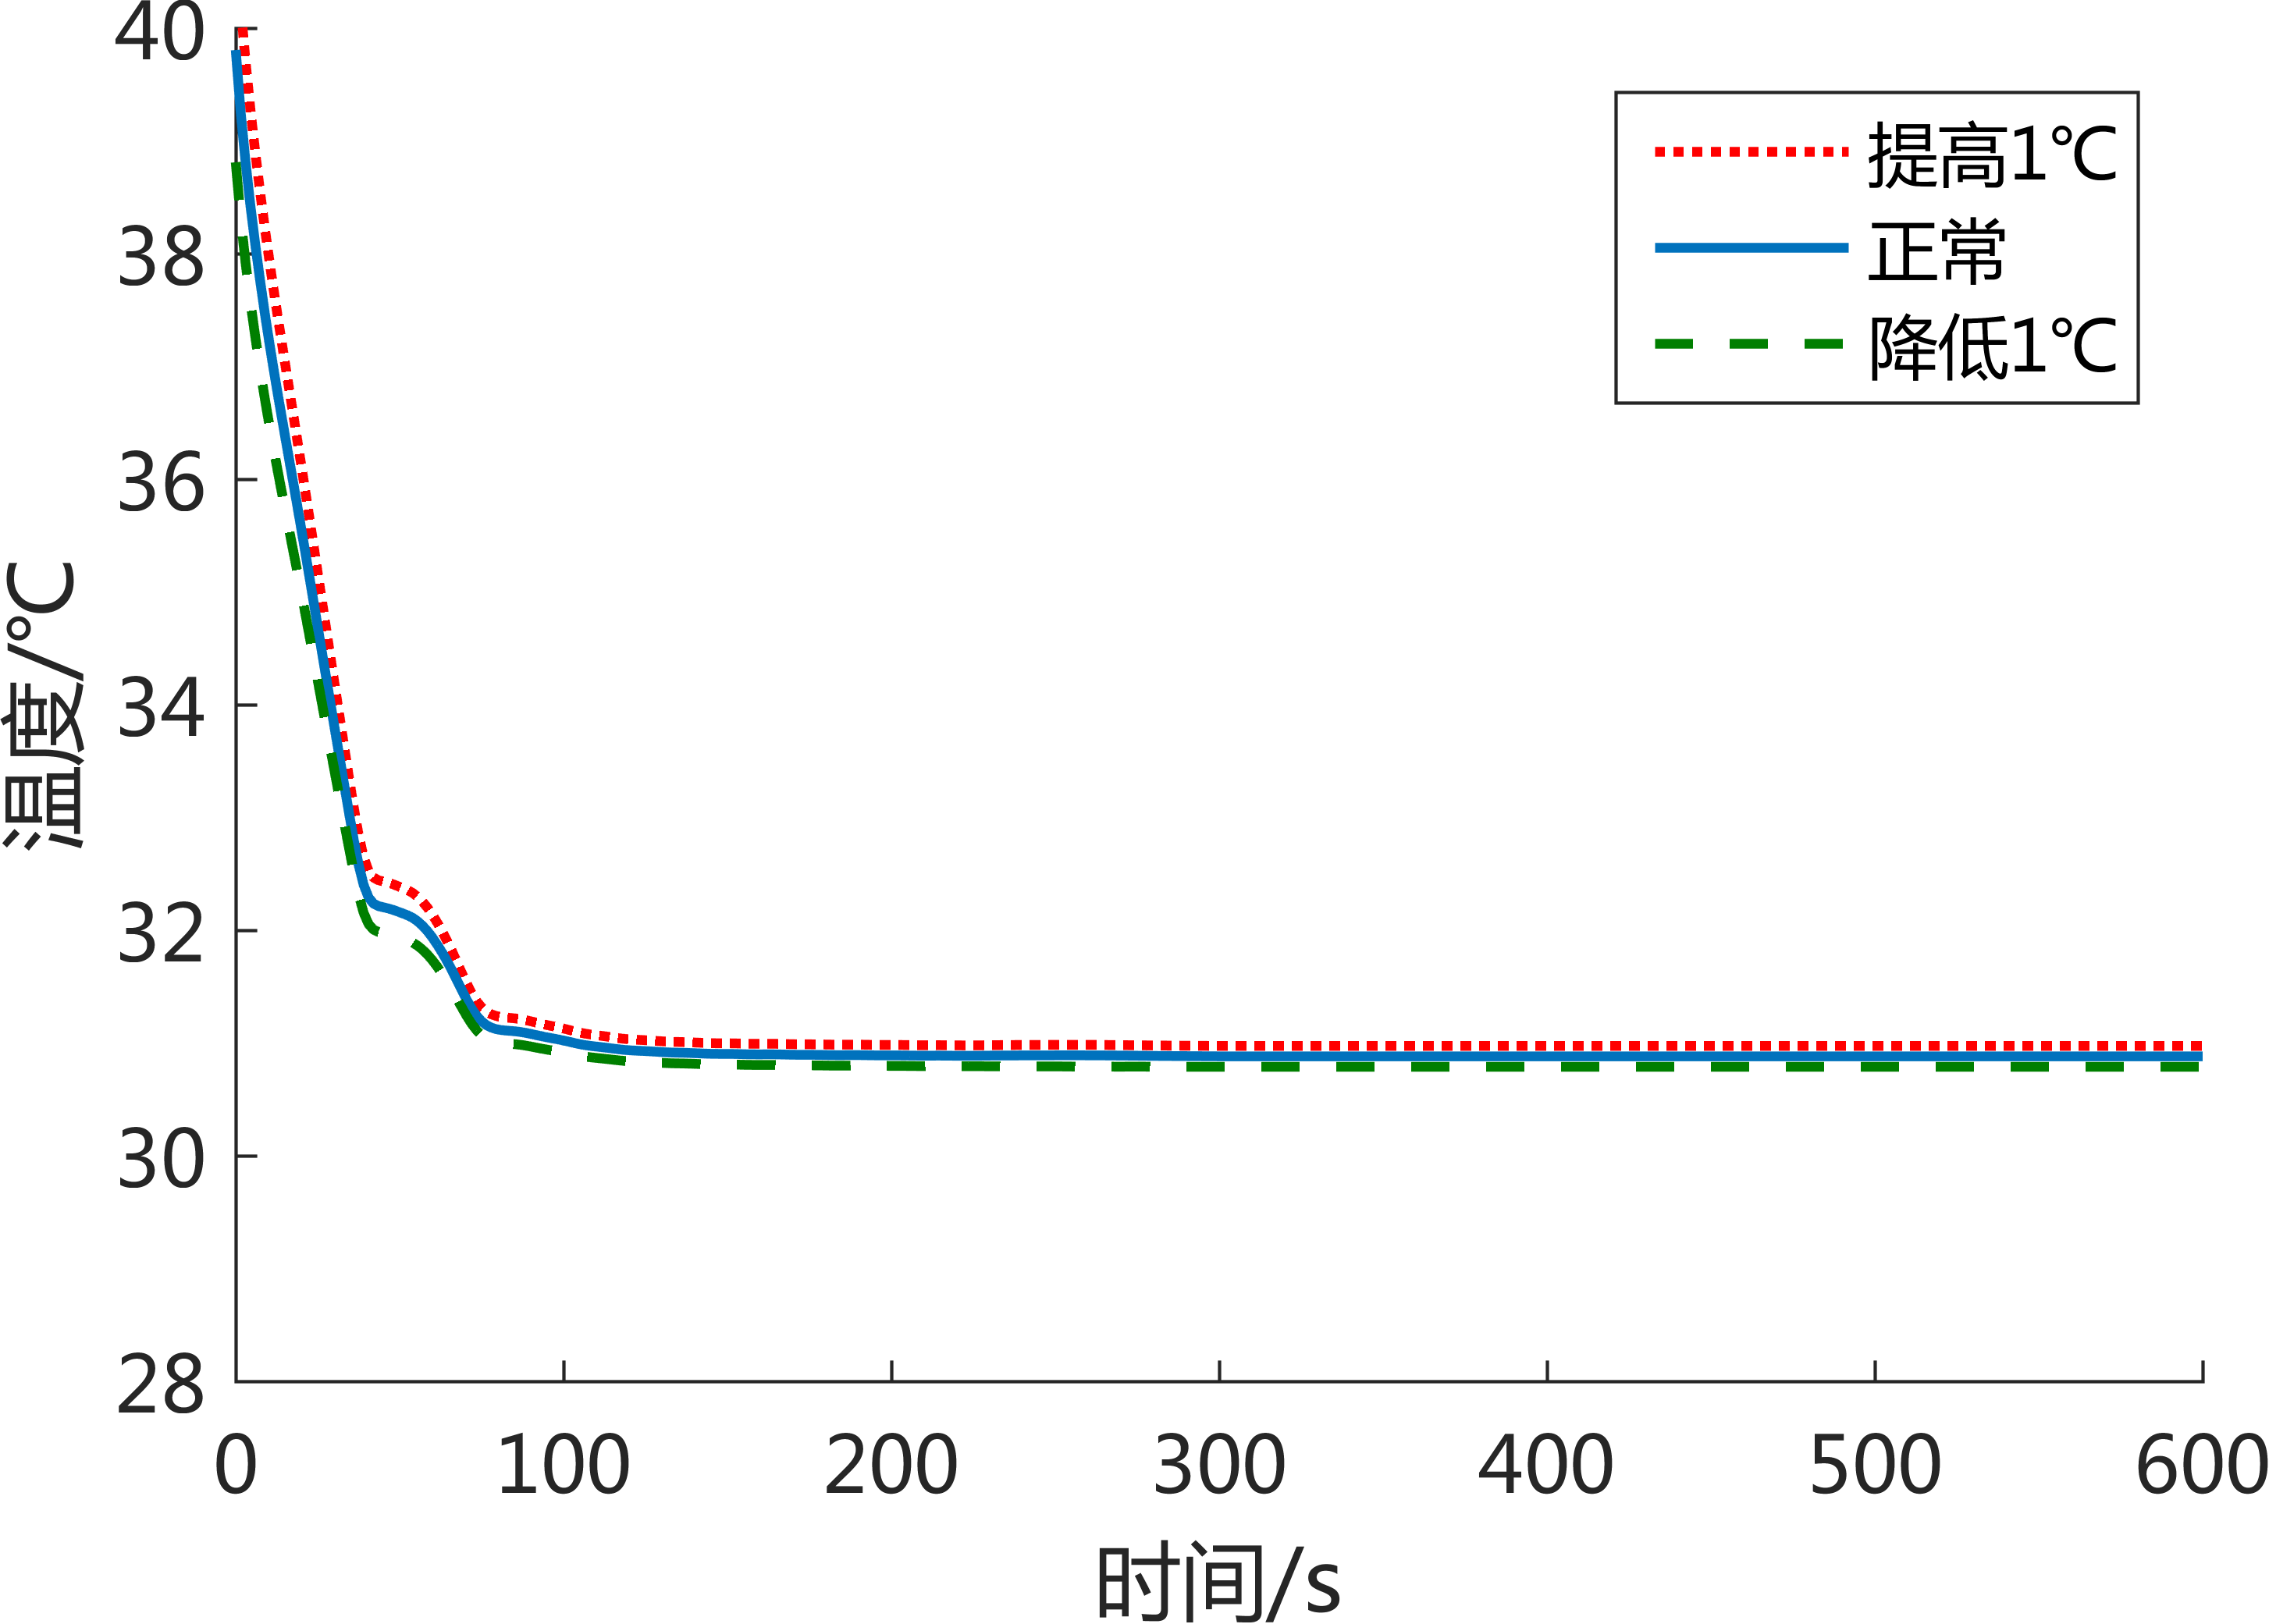
\includegraphics[width=0.4\textwidth]{compare/04.png}
		}
 		\bicaption[fig:Compare]{植物冠层仿真温度与实测温度变化曲线}{植物冠层仿真温度与实测温度变化曲线}{Fig}{Curve of the simulated and measured temperature at Section L}
 	\end{figure}
由\ref{fig:Compare}可知,在空气温度下降阶段,各测点的仿真值相比于对应实测值下降速率明显快,其主要原因是仿真模型是理想的密封环境,而实际温室存在不可避免的空气渗透问题。在稳定阶段两者基本一致,即各个截面的各测点位置的最终稳定温度基本一致。稳定阶段实测值仍会发生小范围内的波动,而仿真值则不会,其主要原因是仿真模型是理想的稳定环境,而实际温室中会存在各种各样不可避免的环境扰动,从而导致温度稳定后仍会发生一定的波动。变化过程中温度梯度也保持一致,即在截面2方向上,距离湿帘越近的位置空气温度下降越早,下降速率也较快,最终达到的稳定温度也较低,第1栋和第2栋温度基本一致,第3栋温度相对较高,且下降速度较慢。
	\begin{figure}[!htp]
		\centering
		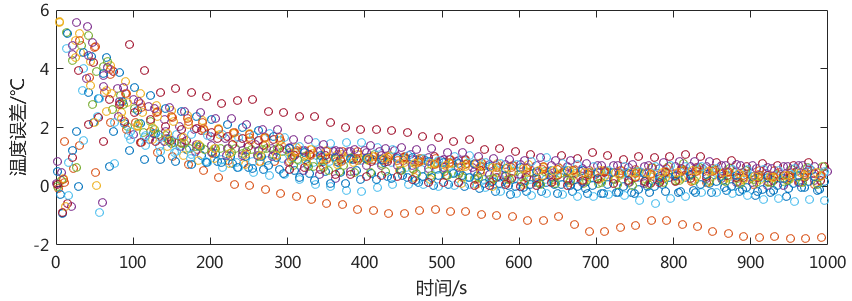
\includegraphics[width=0.8\textwidth]{21error.png}
		\bicaption[fig:Error]{仿真值与实测值绝对误差分布}{仿真值与实测值绝对误差分布}{Fig}{Distribution of absolute error between the simulated and measured temperature}
	\end{figure}
从风机开启至空气温度下降到稳定阶段,温室内所有测点的绝对误差,即实测值与仿真值之差,分布如\ref{fig:Error}所示。由图可知,误差较大的区域主要集中在空气温度快速下降阶段,其主要原因是温室仿真模型和实际温室的差异,即实际温室存在不可避免的空气渗透问题,导致实际情况下空气温度下降速率相较于仿真的理想状态略缓慢,由\ref{fig:Compare}也可观察到这一现象,从而导致在空气温度快速下降阶段误差较大。整个过程均方根误差为1.39℃,平均相对误差为2.63\%,稳定阶段均方根误差为0.53℃,平均相对误差为0.79\%。误差分析结果表明,仿真值和实测值虽存在一定的偏差,但整体温度场的分布和温度变化的趋势基本保持一致。因此,本文所建立的温室CFD仿真模型是有效的,仿真结果能够比较准确的显示温室气温的分布和变化。

\section{机械通风过程分析}
机械通风过程分析以实验条件为例进行分析,实验条件即为表6中的方案1条件,开启风机数量为10台,入口温度为30℃,温室长度为32 m,其它基本参数设置如表5所示。

\ref{fig:V2}所示为实验条件下机械通风过程中截面2的速度瞬态分布云图。从图中可以看出,受机械通风、热浮力共同作用,以及温室边界的限制,温室内气体流动可以看出明显的湍流现象。湿帘入口处空气流动较快,且速度变化较为剧烈,呈现明显的速度梯度,温室内部风速逐渐减弱,温室的上部和边角处速度较小。在机械通风的整个过程,外部空气从湿帘处进入温室从而带动温室内部的空气流动,首先会空气流会在温室内上下波动,达到稳定状态后在风机和湿帘的连线处形成一条空气流,并不断进行小范围内的上下波动。
	\begin{figure}[!htp]
		\centering
		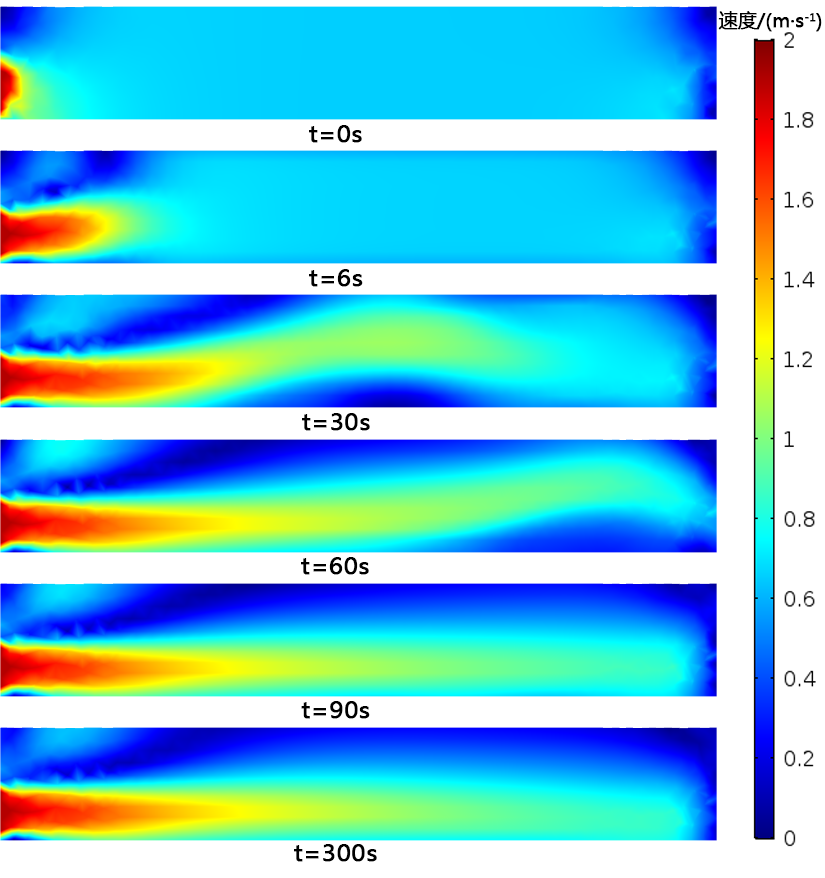
\includegraphics[width=0.5\textwidth]{22V2.png}
		\bicaption[fig:V2]{截面2速度瞬态分布云图}{截面2速度瞬态分布云图}{Fig}{Transient distribution of velocity at Section 2}
	\end{figure}
\ref{fig:VL}所示为实验条件下机械通风过程中截面L的速度瞬态分布云图。可以看出风机出口处空气流动也较快,也呈现出较为明显的速度梯度。另外可以观察到,受温室推拉门的影响,温室中部风速明显较低,且基本不发生变化,通风效果较差。
	\begin{figure}[!htp]
		\centering
		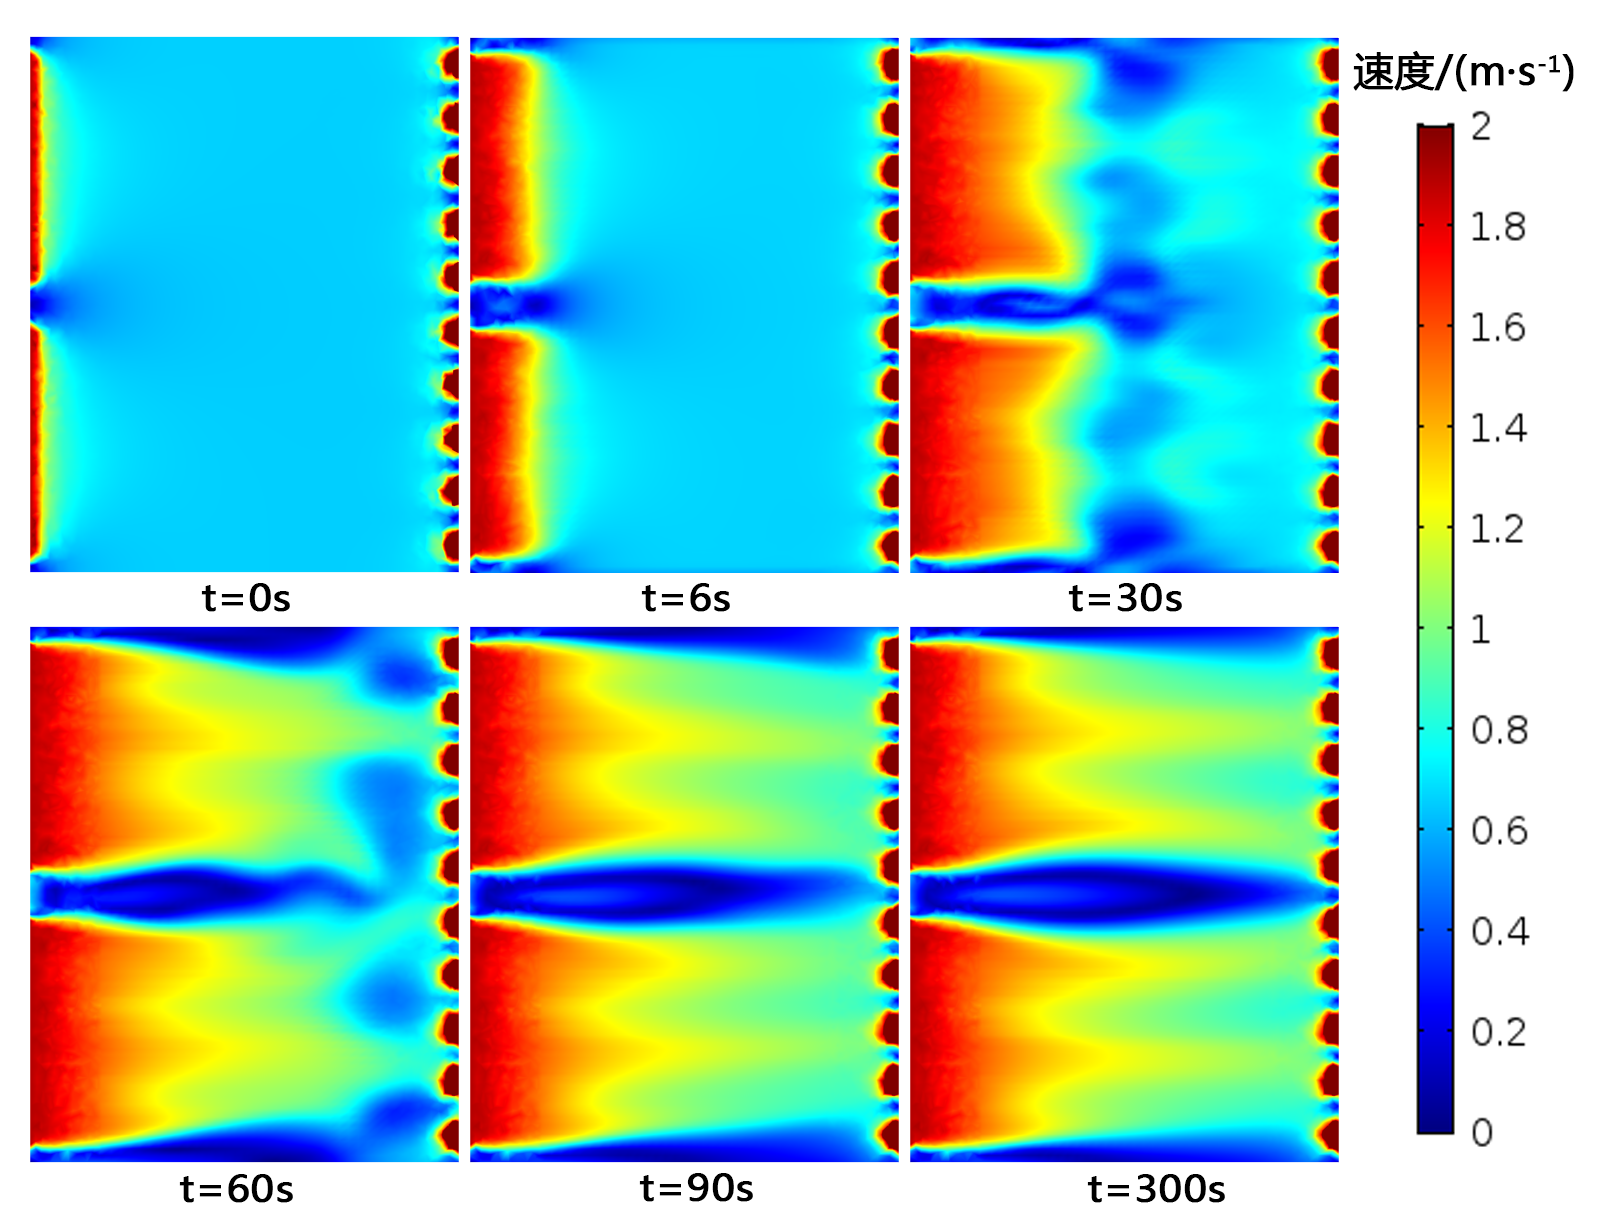
\includegraphics[width=0.8\textwidth]{23VL.png}
		\bicaption[fig:VL]{截面L速度瞬态分布云图}{截面L速度瞬态分布云图}{Fig}{Transient distribution of velocity at Section L}
	\end{figure}
\ref{fig:T2}所示为实验条件下机械通风过程中截面2的温度瞬态分布云图。从图中可以看出:整个通风过程中,地面附近温度相对较高,主要因为这些地方受到强烈的太阳辐射的影响;顶棚附近温度较高,主要因为受太阳辐射和热浮力的共同影响。同时还可以观察到机械通风过程中,风机将温室内热空气抽出产生负压,空气从湿帘处进入温室,经过湿帘将显热转化为潜热形成温度较低的冷空气,形成的冷空气在向前推进的过程中,冷空气会包裹温室内原有的暖空气形成温度漩涡,未及时推动的暖空气会被卷入其中,在冷空气流中不断进行热交换并向前移动,直至到达风机端处排出。
	\begin{figure}[!htp]
		\centering
		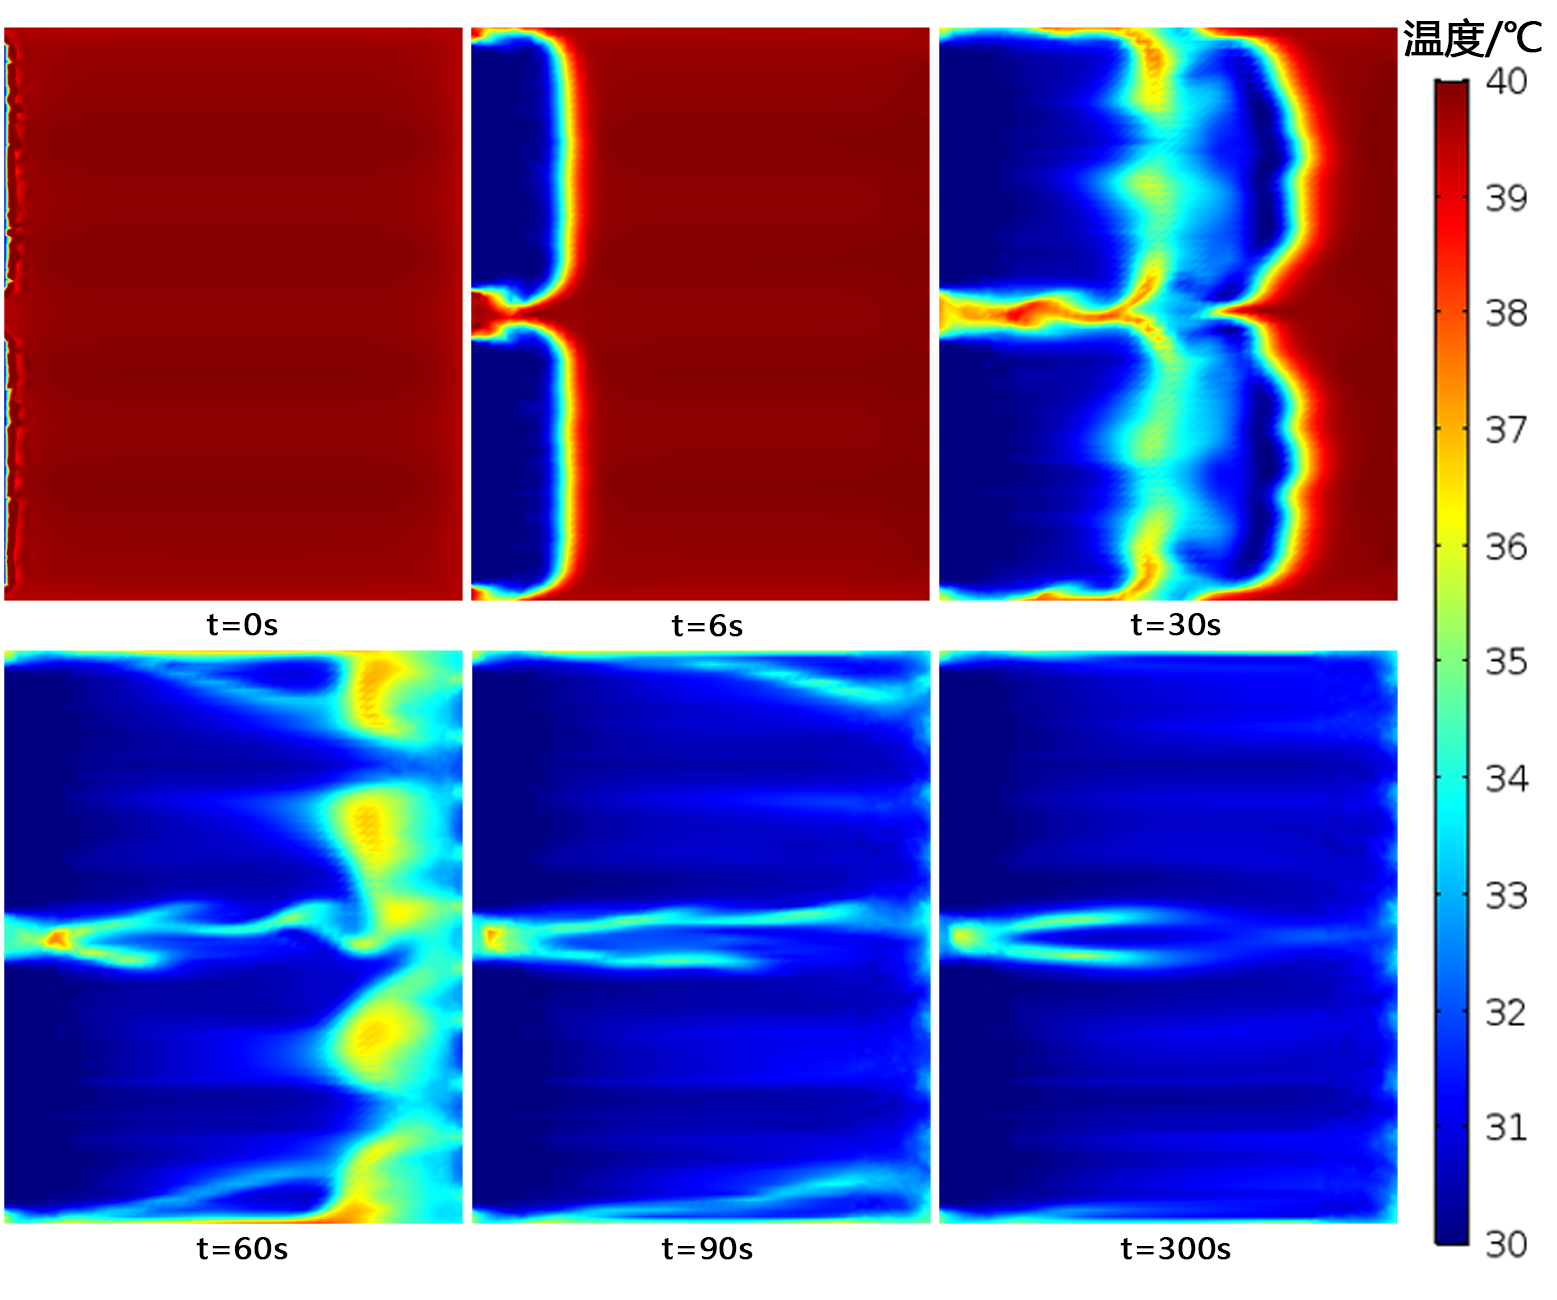
\includegraphics[width=0.5\textwidth]{24T2.png}
		\bicaption[fig:T2]{截面2温度瞬态分布云图}{截面2温度瞬态分布云图}{Fig}{Transient distribution of temperature at Section 2}
	\end{figure}
\ref{fig:VL}所示为实验条件下机械通风过程中截面L的温度瞬态分布云图。从图中可以看出:整个通风过程中,四周壁面附近温度相对较高,主要因为这些地方受到强烈的太阳辐射的影响。由于温度漩涡的存在,水平面上冷空气流在向前推进的过程中会产生断裂,由图28也可观察到这一现象的发生过程。由于气流将热空气携带至风机口处排出,同时受到风机处边界的阻碍,导致风机口处的空气温度相对较高。另外,由于温室中间推拉门的存在,形成了两套湿帘之间的不连续,从而使温室水平方向中间部分的通风效果较差,导致该区域的降温效果也较差。在\ref{fig:T2}和\ref{fig:TL}中还可以看出,受温室边界及热浮力的影响,温室各角落温度相对较高。
	\begin{figure}[!htp]
		\centering
		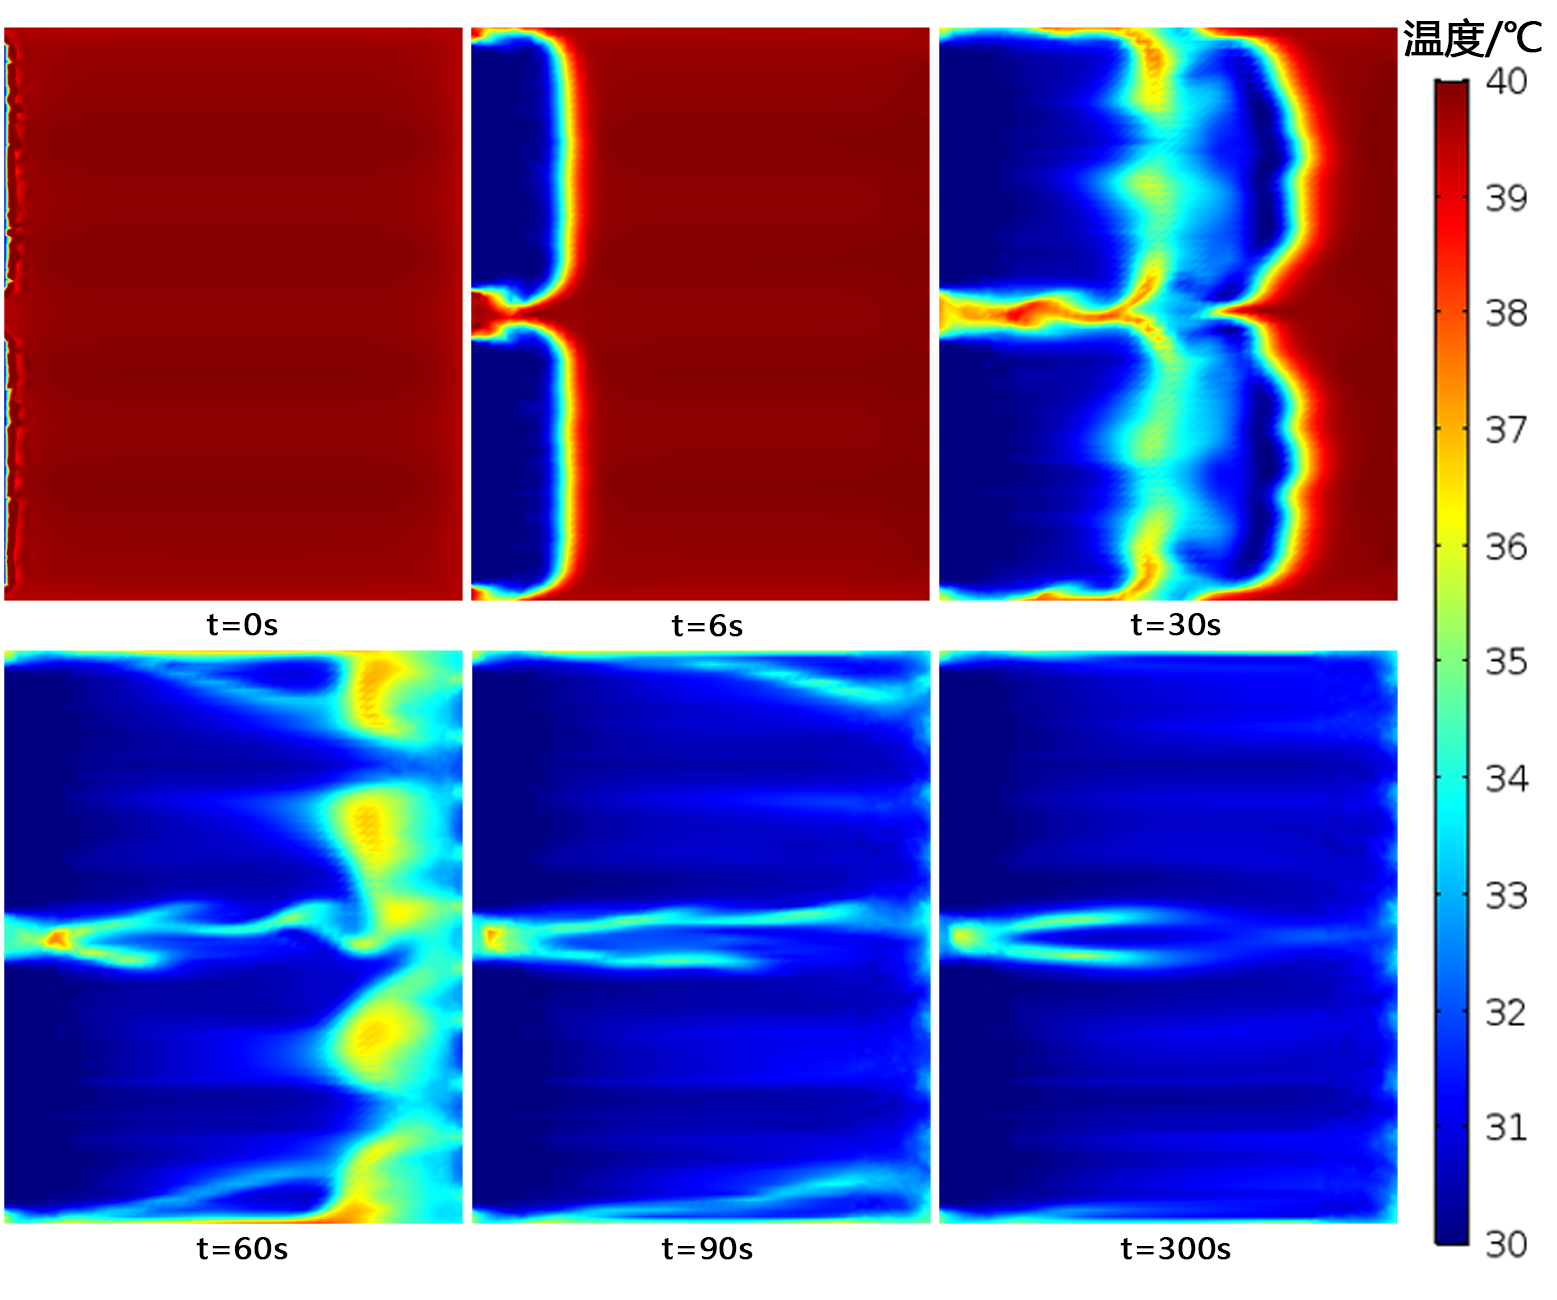
\includegraphics[width=0.8\textwidth]{25TL.png}
		\bicaption[fig:TL]{截面L温度瞬态分布云图}{截面L温度瞬态分布云图}{Fig}{Transient distribution of temperature at Section L}
	\end{figure}
\section{本章小结}
本章针对机械通风降温而带来的能源消耗、生产成本较高的问题,和温室面积大带来的监测点较多、监测成本较高的问题,建立温室CFD仿真模型,对温室机械通风过程进行分析,为温室优化结构参数和通风设备配置,为基于农业物联网的智能温室监测与控制系统提供优化的监测点位置选择和机械通风控制策略。

本章首先阐述分析了温室CFD仿真的概况和研究意义。然后对CFD仿真的理论基础进行了简单阐述,选择COMSOL Multiphysics多物理场仿真软件进行温室CFD仿真建模,并对温室仿真模型进行了几何建模、多物理场选择、边界条件设置、网格划分和求解。

为了验证仿真模型的有效性和可靠性,本章基于智能温室监测与控制系统进行了夏季温室机械通风实验,并详细说明了本次通风实验的实验方案和实验步骤,然后将实验结果和仿真结果进行了对比分析,验证了仿真模型瞬态和稳态计算的准确性和有效性。

最后本章基于已经验证的温室仿真模型对温室的机械通风过程进行了分析,得到了机械通风过程中温室内空气流动的规律和空气温度的分布和变化规律。

本章所建立的温室仿真模型虽然是针对本文实验温室建立,但是建立仿真模型的原理和方法是通用的,可针对任意温室修改几何模型和边界条件设置,重新划分网格即可进行仿真分析;同理,本文的模型虽然是针对夏季温室机械通风建立,但是可对边界条件进行一定的修改即可对其它条件下的温室稳态和瞬态过程进行分析。